\documentclass[aspectratio=169,10pt]{beamer}
\usepackage{tikz}
\usetikzlibrary{arrows.meta,positioning,calc,fit,backgrounds,shapes.geometric}

\definecolor{Navy}{HTML}{183B56}
\definecolor{Blue}{HTML}{2F75B5}
\definecolor{BlueLight}{HTML}{DDEBF7}
\definecolor{Orange}{HTML}{E67E22}
\definecolor{OrangeLight}{HTML}{FCE4D6}
\definecolor{Purple}{HTML}{7030A0}
\definecolor{Green}{HTML}{548235}
\definecolor{Gray}{HTML}{606060}
\definecolor{GrayLight}{HTML}{F2F2F2}

\setbeamercolor{background canvas}{bg=white}
\setbeamercolor{frametitle}{fg=Navy,bg=white}
\setbeamerfont{frametitle}{series=\bfseries,size=\large}
\setbeamertemplate{navigation symbols}{}
\setbeamertemplate{footline}{}

\tikzset{
  block/.style={draw=Navy,fill=BlueLight,rounded corners=2pt,minimum width=1.45cm,minimum height=.72cm,align=center,font=\small\sffamily},
  smallblock/.style={draw=Navy,fill=BlueLight,rounded corners=2pt,minimum width=1.05cm,minimum height=.55cm,align=center,font=\scriptsize\sffamily},
  mux/.style={draw=Purple,fill=white,trapezium,trapezium left angle=70,trapezium right angle=110,minimum width=.78cm,minimum height=1.05cm,align=center,font=\scriptsize\sffamily},
  pg/.style={draw=Blue,fill=BlueLight,rectangle,minimum width=.7cm,minimum height=.55cm,align=center,font=\scriptsize\sffamily},
  prefnode/.style={draw=Navy,fill=Navy,circle,minimum size=.27cm,inner sep=0pt},
  grayprefix/.style={draw=Navy,fill=white,circle,minimum size=.27cm,inner sep=0pt},
  data/.style={-{Latex[length=2.2mm]},draw=Navy,thick},
  carry/.style={-{Latex[length=2.2mm]},draw=Orange,very thick},
  control/.style={-{Latex[length=2.2mm]},draw=Purple,thick,dashed},
  note/.style={font=\scriptsize\sffamily,text=Gray,align=center},
  label/.style={font=\small\sffamily,text=Navy}
}

\begin{document}

% 1. Ripple Carry Adder
\begin{frame}{Ripple Carry Adder (RCA): carry propagates stage by stage}
\centering
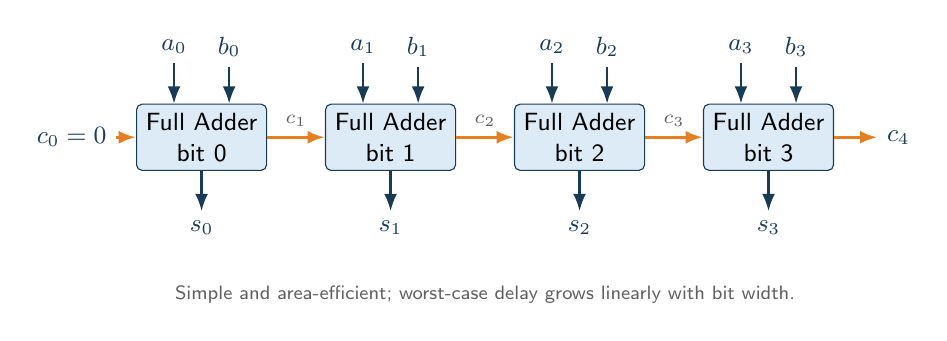
\begin{tikzpicture}[x=1cm,y=1cm]
  \foreach \i/\x in {0/-3.6,1/-1.2,2/1.2,3/3.6}{
    \node[block] (fa\i) at (\x,0) {Full Adder\\bit \i};
    \node[label] (a\i) at ($(fa\i.north)+(-.35,.72)$) {$a_{\i}$};
    \node[label] (b\i) at ($(fa\i.north)+(.35,.72)$) {$b_{\i}$};
    \draw[data] (a\i) -- ($(fa\i.north)+(-.35,0)$);
    \draw[data] (b\i) -- ($(fa\i.north)+(.35,0)$);
    \node[label] (s\i) at ($(fa\i.south)+(0,-.72)$) {$s_{\i}$};
    \draw[data] (fa\i.south) -- (s\i);
  }
  \node[label] (cin) at (-5.25,0) {$c_0=0$};
  \draw[carry] (cin) -- (fa0.west);
  \draw[carry] (fa0.east) -- node[above,note] {$c_1$} (fa1.west);
  \draw[carry] (fa1.east) -- node[above,note] {$c_2$} (fa2.west);
  \draw[carry] (fa2.east) -- node[above,note] {$c_3$} (fa3.west);
  \node[label] (cout) at (5.25,0) {$c_4$};
  \draw[carry] (fa3.east) -- (cout);
  \node[note] at (0,-2.0) {Simple and area-efficient; worst-case delay grows linearly with bit width.};
\end{tikzpicture}
\end{frame}

% 2. Carry Lookahead Adder
\begin{frame}{Carry Lookahead Adder (CLA): compute carries in parallel}
\centering
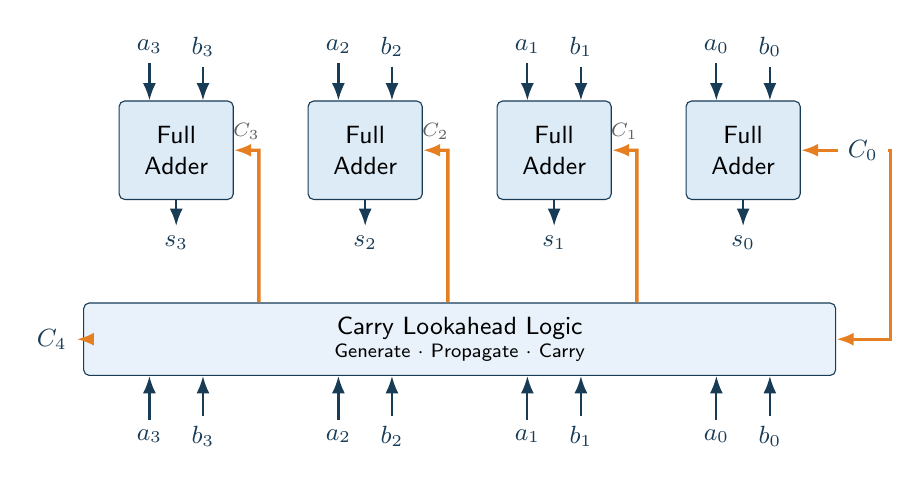
\begin{tikzpicture}[x=1cm,y=1cm]
  \foreach \i/\x in {3/-3.6,2/-1.2,1/1.2,0/3.6}{
    \node[block,minimum width=1.45cm,minimum height=1.25cm] (fa\i) at (\x,.85)
      {Full\\Adder};
    \node[label] (a\i) at ($(fa\i.north)+(-.34,.68)$) {$a_{\i}$};
    \node[label] (b\i) at ($(fa\i.north)+(.34,.68)$) {$b_{\i}$};
    \draw[data] (a\i) -- ($(fa\i.north)+(-.34,0)$);
    \draw[data] (b\i) -- ($(fa\i.north)+(.34,0)$);
    \node[label] (s\i) at ($(fa\i.south)+(0,-.54)$) {$s_{\i}$};
    \draw[data] (fa\i.south) -- (s\i);
  }

  \node[block,fill=BlueLight!65,minimum width=9.55cm,minimum height=.92cm] (look) at (0,-1.55)
    {Carry Lookahead Logic\\[-1mm]\scriptsize Generate $\boldsymbol{\cdot}$ Propagate $\boldsymbol{\cdot}$ Carry};

  % The lookahead network supplies C1--C3 directly to the corresponding
  % full-adder stages instead of passing them through a ripple chain.
  \coordinate (c3tap) at (-2.55,-1.08);
  \coordinate (c2tap) at (-.15,-1.08);
  \coordinate (c1tap) at (2.25,-1.08);
  \draw[carry] (c3tap) -- ++(0,1.93) -- node[above,note] {$C_3$} (fa3.east);
  \draw[carry] (c2tap) -- ++(0,1.93) -- node[above,note] {$C_2$} (fa2.east);
  \draw[carry] (c1tap) -- ++(0,1.93) -- node[above,note] {$C_1$} (fa1.east);

  \node[label] (cin) at (5.12,.85) {$C_0$};
  \draw[carry] (cin) -- (fa0.east);
  \draw[carry] (cin) -- ++(.35,0) |- (look.east);
  \node[label] (cout) at (-5.18,-1.55) {$C_4$};
  \draw[carry] (look.west) -- (cout);

  % Operand bits also feed the generate/propagate logic, as in the reference
  % block diagram. They are repeated below to keep the signal flow legible.
  \foreach \i/\x in {3/-3.6,2/-1.2,1/1.2,0/3.6}{
    \node[label] (al\i) at (\x-.34,-2.78) {$a_{\i}$};
    \node[label] (bl\i) at (\x+.34,-2.78) {$b_{\i}$};
    \draw[data] (al\i) -- (look.south -| al\i);
    \draw[data] (bl\i) -- (look.south -| bl\i);
  }
\end{tikzpicture}
\end{frame}

% 3. Carry Select Adder
\begin{frame}{Carry Select Adder (CSA)}
\centering
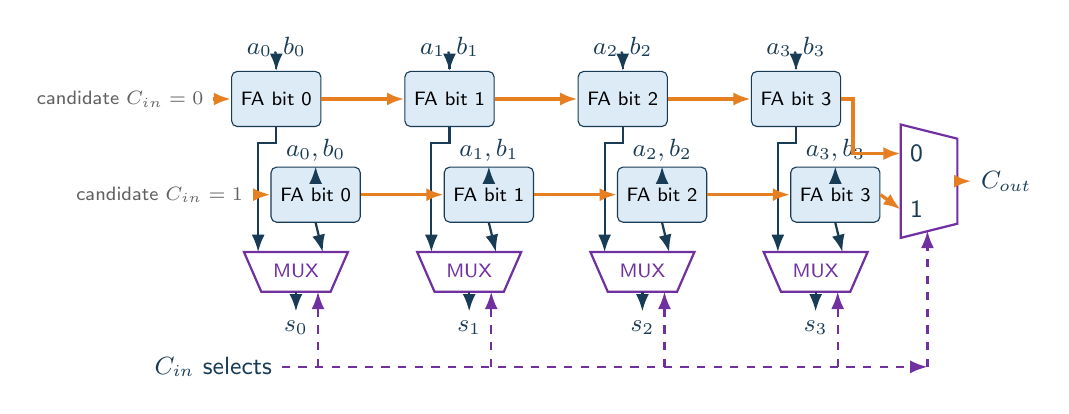
\begin{tikzpicture}[x=1cm,y=.90cm]
  % Two complete carry chains are evaluated in parallel. The upper row
  % assumes carry-in 0 and the lower row assumes carry-in 1.
  \foreach \i/\x in {0/-3.3,1/-1.1,2/1.1,3/3.3}{
    \node[smallblock,minimum width=1.12cm,minimum height=.70cm] (fa0\i) at (\x-.25,1.30)
      {FA bit \i};
    \node[smallblock,minimum width=1.12cm,minimum height=.70cm] (fa1\i) at (\x+.25,-.05)
      {FA bit \i};

    \node[label] (ab0\i) at (\x-.25,2.02) {$a_{\i},b_{\i}$};
    \node[label] (ab1\i) at (\x+.25,.58) {$a_{\i},b_{\i}$};
    \draw[data] (ab0\i) -- (fa0\i.north);
    \draw[data] (ab1\i) -- (fa1\i.north);

    % Downward sum mux: upper candidate enters on the left, lower candidate
    % on the right, and the selected sum leaves at the bottom.
    \coordinate (smul\i) at (\x-.66,-.86);
    \coordinate (smur\i) at (\x+.66,-.86);
    \coordinate (smlr\i) at (\x+.44,-1.42);
    \coordinate (smll\i) at (\x-.44,-1.42);
    \path[draw=Purple,fill=white,thick]
      (smul\i) -- (smur\i) -- (smlr\i) -- (smll\i) -- cycle;
    \node[note,text=Purple] at (\x,-1.13) {MUX};

    \draw[data] (fa0\i.south) -- ++(0,-.22) -| (\x-.48,-.86);
    \draw[data] (fa1\i.south) -- (\x+.34,-.86);
    \node[label] (sum\i) at (\x,-1.93) {$s_{\i}$};
    \draw[data] (\x,-1.42) -- (sum\i);
  }

  \node[note,anchor=east] (zero) at (-4.35,1.30) {candidate $C_{in}=0$};
  \node[note,anchor=east] (one) at (-3.85,-.05) {candidate $C_{in}=1$};
  \draw[carry] (zero.east) -- (fa00.west);
  \draw[carry] (one.east) -- (fa10.west);
  \foreach \i/\j in {0/1,1/2,2/3}{
    \draw[carry] (fa0\i.east) -- (fa0\j.west);
    \draw[carry] (fa1\i.east) -- (fa1\j.west);
  }

  % The final mux chooses the candidate carry-out. All signal flow remains
  % left-to-right, matching the requested orientation.
  \coordinate (cmul) at (4.38,.94);
  \coordinate (cmur) at (5.10,.74);
  \coordinate (cmlr) at (5.10,-.46);
  \coordinate (cmll) at (4.38,-.66);
  \path[draw=Purple,fill=white,thick] (cmul) -- (cmur) -- (cmlr) -- (cmll) -- cycle;
  \node[label] at (4.58,.53) {0};
  \node[label] at (4.58,-.26) {1};
  \draw[carry] (fa03.east) -- ++(.15,0) |- (4.38,.53);
  \draw[carry] (fa13.east) -- (4.38,-.26);
  \node[label] (cout) at (5.72,.14) {$C_{out}$};
  \draw[carry] (5.10,.14) -- (cout);

  % The real carry-in selects all four sum bits and the final carry.
  \node[label] (select) at (-4.35,-2.48) {$C_{in}$ selects};
  \draw[control] (select) -- (4.72,-2.48);
  \foreach \x in {-3.3,-1.1,1.1,3.3}{
    \draw[control] (\x+.28,-2.48) -- (\x+.28,-1.42);
  }
  \draw[control] (4.72,-2.48) -- (4.72,-.56);
\end{tikzpicture}
\end{frame}

% 4. Carry Skip Adder
\begin{frame}{Carry Skip Adder (CSkipA)}
\centering
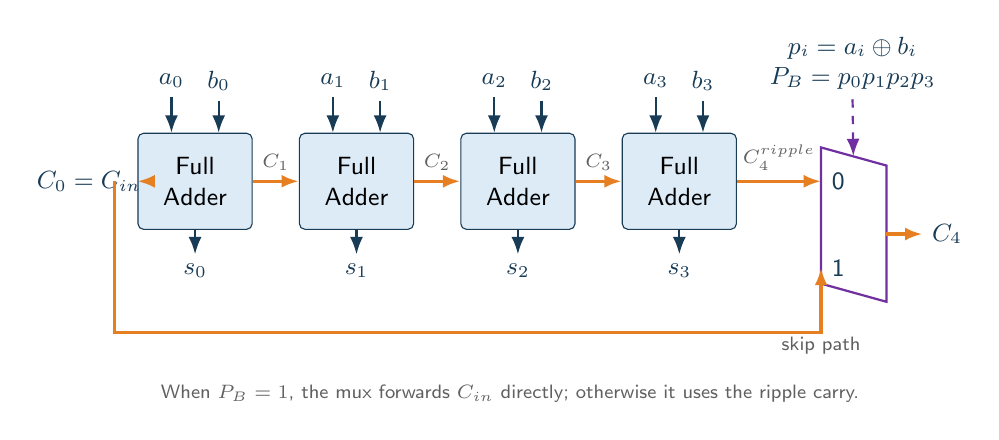
\begin{tikzpicture}[x=1cm,y=1cm]
  \foreach \i/\x in {0/-4.0,1/-1.95,2/.10,3/2.15}{
    \node[block,minimum width=1.45cm,minimum height=1.22cm] (fa\i) at (\x,.55)
      {Full\\Adder};
    \node[label] (a\i) at ($(fa\i.north)+(-.30,.66)$) {$a_{\i}$};
    \node[label] (b\i) at ($(fa\i.north)+(.30,.66)$) {$b_{\i}$};
    \draw[data] (a\i) -- ($(fa\i.north)+(-.30,0)$);
    \draw[data] (b\i) -- ($(fa\i.north)+(.30,0)$);
    \node[label] (s\i) at ($(fa\i.south)+(0,-.52)$) {$s_{\i}$};
    \draw[data] (fa\i.south) -- (s\i);
  }

  \node[label] (cin) at (-5.35,.55) {$C_0=C_{in}$};
  \draw[carry] (cin) -- (fa0.west);
  \draw[carry] (fa0.east) -- node[above,note] {$C_1$} (fa1.west);
  \draw[carry] (fa1.east) -- node[above,note] {$C_2$} (fa2.west);
  \draw[carry] (fa2.east) -- node[above,note] {$C_3$} (fa3.west);

  % A narrow, vertical carry mux matching the conventional carry-skip block
  % diagram: ripple carry enters at input 0 and bypass carry at input 1.
  \coordinate (muxul) at (3.95,.98);
  \coordinate (muxur) at (4.78,.75);
  \coordinate (muxlr) at (4.78,-.98);
  \coordinate (muxll) at (3.95,-.75);
  \path[draw=Purple,fill=white,thick] (muxul) -- (muxur) -- (muxlr) -- (muxll) -- cycle;
  \coordinate (muxzero) at (3.95,.55);
  \coordinate (muxone) at (3.95,-.55);
  \coordinate (muxselect) at (4.36,.87);
  \coordinate (muxout) at (4.78,-.12);
  \node[label] at (4.17,.55) {0};
  \node[label] at (4.17,-.55) {1};
  \draw[carry] (fa3.east) -- node[above,note] {$C_4^{ripple}$} (muxzero);
  \node[label] (cout) at (5.55,-.12) {$C_4$};
  \draw[carry] (muxout) -- (cout);

  % If all four bits propagate, the incoming carry takes the lower bypass
  % input of the mux instead of waiting for the four-stage ripple path.
  \coordinate (cinbranch) at (-5.02,.55);
  \draw[carry] (cinbranch) -- ++(0,-1.92) -| node[below,note,pos=.55] {skip path} (muxone);
  \node[label,align=center] (propagate) at (4.35,2.05)
    {$p_i=a_i\oplus b_i$\\$P_B=p_0p_1p_2p_3$};
  \draw[control] (propagate.south) -- (muxselect);
  \node[note] at (0,-2.15) {When $P_B=1$, the mux forwards $C_{in}$ directly; otherwise it uses the ripple carry.};
\end{tikzpicture}
\end{frame}

% 5. Kogge-Stone Adder
\begin{frame}{Kogge--Stone Adder (KSA): parallel-prefix carry tree}
\centering
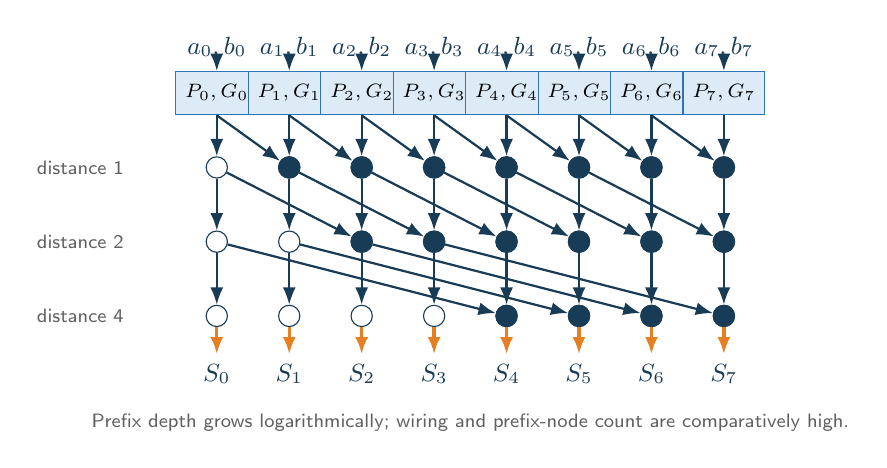
\begin{tikzpicture}[x=.92cm,y=.82cm]
  \foreach \i in {0,...,7}{
    \pgfmathsetmacro{\x}{\i-3.5}
    \node[pg] (p\i) at (\x,2.25) {$P_{\i},G_{\i}$};
    \node[label] at (\x,2.95) {$a_{\i},b_{\i}$};
    \draw[data] (\x,2.85) -- (p\i.north);
  }
  \foreach \i in {0,...,7}{
    \pgfmathsetmacro{\x}{\i-3.5}
    \node[grayprefix] (s1\i) at (\x,1.10) {};
    \draw[data] (p\i.south) -- (s1\i);
  }
  \foreach \i in {1,...,7}{
    \pgfmathtruncatemacro{\j}{\i-1}
    \draw[data] (p\j.south) -- (s1\i);
    \node[prefnode] at (s1\i) {};
  }
  \foreach \i in {0,...,7}{
    \pgfmathsetmacro{\x}{\i-3.5}
    \node[grayprefix] (s2\i) at (\x,-.05) {};
    \draw[data] (s1\i) -- (s2\i);
  }
  \foreach \i in {2,...,7}{
    \pgfmathtruncatemacro{\j}{\i-2}
    \draw[data] (s1\j) -- (s2\i);
    \node[prefnode] at (s2\i) {};
  }
  \foreach \i in {0,...,7}{
    \pgfmathsetmacro{\x}{\i-3.5}
    \node[grayprefix] (s3\i) at (\x,-1.20) {};
    \draw[data] (s2\i) -- (s3\i);
  }
  \foreach \i in {4,...,7}{
    \pgfmathtruncatemacro{\j}{\i-4}
    \draw[data] (s2\j) -- (s3\i);
    \node[prefnode] at (s3\i) {};
  }
  \foreach \i in {0,...,7}{
    \pgfmathsetmacro{\x}{\i-3.5}
    \node[label] (sum\i) at (\x,-2.10) {$S_{\i}$};
    \draw[carry] (s3\i) -- (sum\i);
  }
  \node[note,anchor=east] at (-4.65,1.10) {distance 1};
  \node[note,anchor=east] at (-4.65,-.05) {distance 2};
  \node[note,anchor=east] at (-4.65,-1.20) {distance 4};
  \node[note] at (0,-2.85) {Prefix depth grows logarithmically; wiring and prefix-node count are comparatively high.};
\end{tikzpicture}
\end{frame}

% 6. Hybrid Adder
\begin{frame}{Hybrid Adder (HA8): combine CLA and Kogge--Stone blocks}
\centering
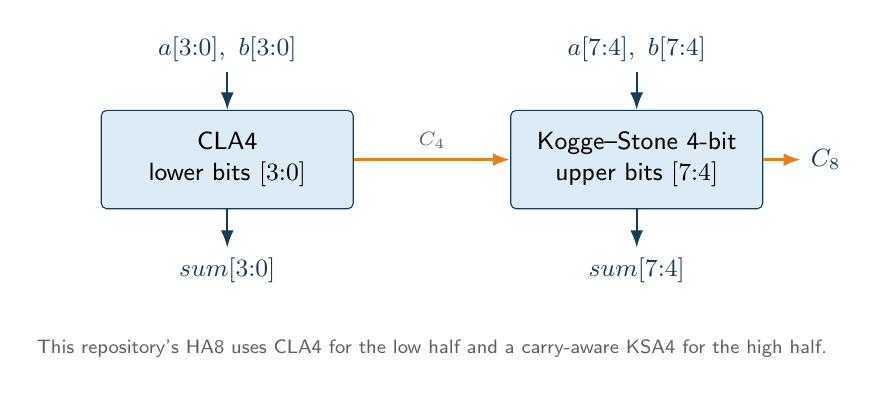
\begin{tikzpicture}[x=1cm,y=1cm]
  \node[block,minimum width=3.2cm,minimum height=1.25cm] (cla) at (-2.6,.25)
    {CLA4\\lower bits $[3{:}0]$};
  \node[block,minimum width=3.2cm,minimum height=1.25cm] (ksa) at (2.6,.25)
    {Kogge--Stone 4-bit\\upper bits $[7{:}4]$};
  \node[label] (lo) at (-2.6,1.65) {$a[3{:}0],\ b[3{:}0]$};
  \node[label] (hi) at (2.6,1.65) {$a[7{:}4],\ b[7{:}4]$};
  \draw[data] (lo) -- (cla.north);
  \draw[data] (hi) -- (ksa.north);
  \node[label] (slo) at (-2.6,-1.15) {$sum[3{:}0]$};
  \node[label] (shi) at (2.6,-1.15) {$sum[7{:}4]$};
  \draw[data] (cla.south) -- (slo);
  \draw[data] (ksa.south) -- (shi);
  \draw[carry] (cla.east) -- node[above,note] {$C_4$} (ksa.west);
  \node[label] (cout) at (5.0,.25) {$C_8$};
  \draw[carry] (ksa.east) -- (cout);
  \node[note] at (0,-2.15) {This repository's HA8 uses CLA4 for the low half and a carry-aware KSA4 for the high half.};
\end{tikzpicture}
\end{frame}

\end{document}
